\subsection{Simulation-Based Jet Background Cuts and Efficiencies}
\label{sec:sim_jet_background}

A necessary step in the analysis is the removal of “jet background,” defined as non-collision background events that are mistakenly reconstructed as jets. 
The primary sources of non-collision background observed in sPHENIX data arise from two sources: upstream beam backgrounds and cosmic rays. The upstream beam background are typically observed as muons traveling along the beam axis and the showering cosmic ray background is usually observed traveling vertically through the detector. 
In principle, many of these backgrounds can be removed by matching calorimeter tower jets to tracks, as is done in other heavy ion experiments. However, tracking information is not available for the majority of the p+p jet data collected in Run 2024.

The two methods are considered for background rejection~\cite{ppg09AN}:
\begin{itemize}
    \item The first method, referred to as the “energy fraction" requirement, applies selections on the fraction of reconstructed jet energy deposited in each calorimeter layer. Specifically, the EMCal and OHCal fractions, $E_{EMCal}/E_{Jet}$ and $E_{OHCal}/E_{Jet}$, must be between 10\% and 90\%, while the IHCal fraction, $E_{IHCal}/E_{Jet}$, must lie between 0\% and 90\%. Notably, this method would require a simulation-based correction for this jet selection inefficiency and is therefore sensitive to the \geant modeling of the longitudinal shower deposition in simulation.
    \item The second method, the “dijet" requirement, necessitates the presence of a second jet in the event, approximately balanced in azimuth. Specifically, the ratio of the subleading jet energy to the leading jet energy must exceed 0.3, and the azimuthal separation ($\delta\phi$) must be greater than 3$\pi$/4. This method would also require a simulation-based correction for this jet selection inefficiency and is instead sensitive to the modeling of dijet topologies in the event generator, \pythia.
\end{itemize}

These background rejection strategies are first studied in \pythia + \geant simulation to assess their impact on the underlying event (UE) measurement. 
Figures~\ref{fig:sim_efrac_bkg_tr_et} and~\ref{fig:sim_dijet_bkg_tr_et} show the effect of the energy fraction and dijet selections, respectively, on the transverse region $E_{T}$ distribution. 
The energy fraction requirement does not introduce a significant bias in the reconstructed UE measurement, while the dijet selection leads to a small bias at the 5--10\% level.

Based on these studies, the "energy fraction" requirement is used as the primary simulation-driven jet background rejection method. 
The impact of the energy fraction requirement on the reconstructed jet $p_{T}$ distribution in the analysis range is shown in Figure~\ref{fig:sim_efrac_bkg_jetpt}.
In addition, data-driven timing cuts are developed and applied to further suppress residual backgrounds not removed by the energy fraction selection. 
These data-driven timing cuts are discussed in more detail in the follow sections.

\begin{figure}
    \centering
    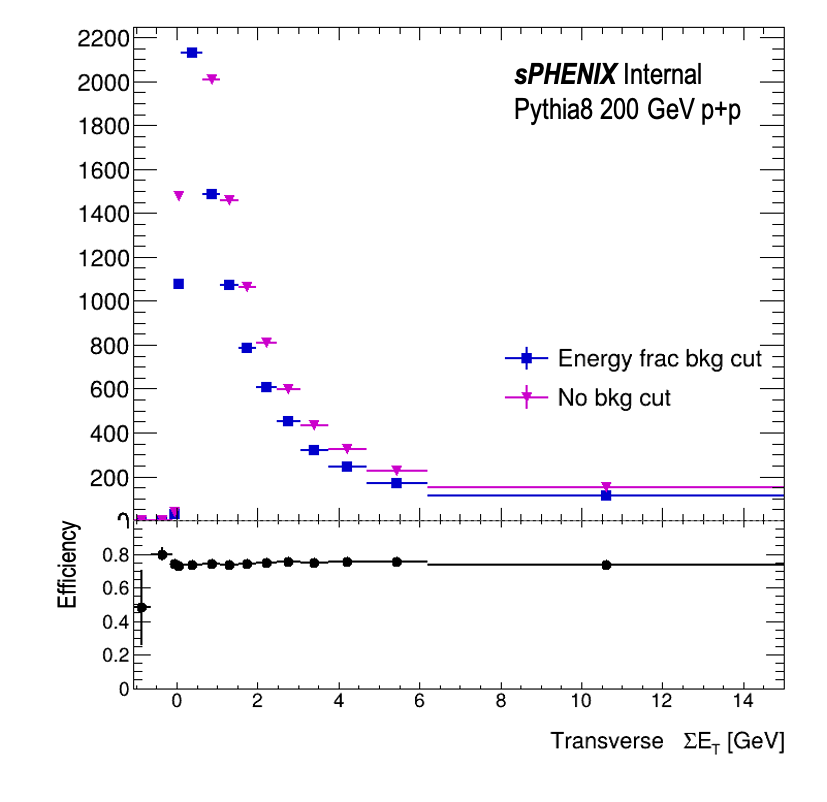
\includegraphics[width=0.48\linewidth]{figures/chapter5/efrac_bkg_cut_efficiency.png}
    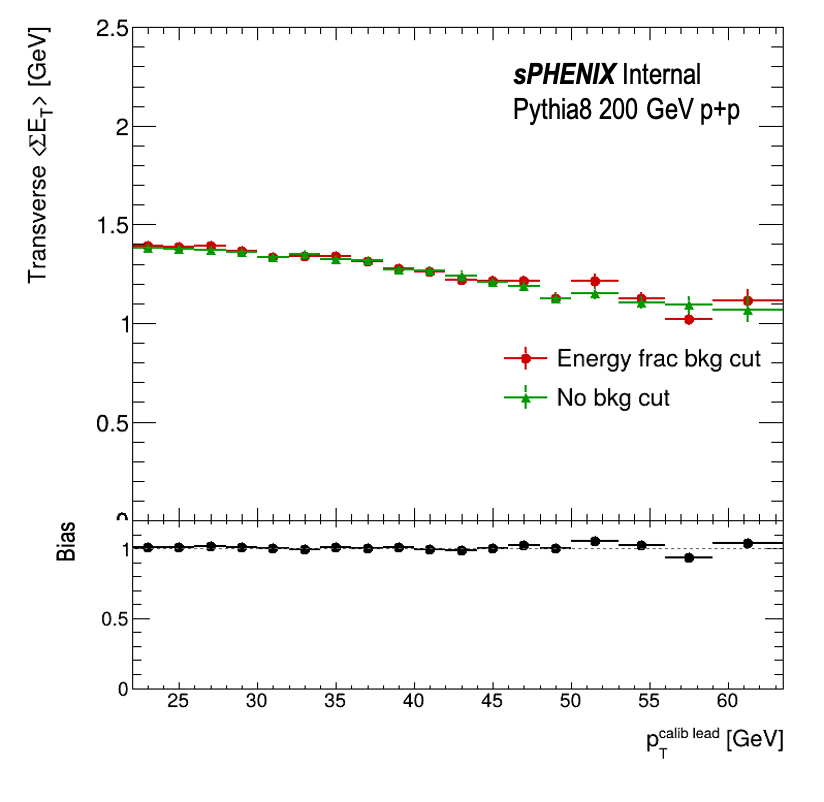
\includegraphics[width=0.48\linewidth]{figures/chapter5/efrac_bkg_cut_bias.png}
    \caption{Effect of the energy fraction cut on the transverse region $E_{T}$ distribution in the \pythia simulation dataset. 
    The left plot shows the efficiency of the energy fraction background cut application on the reco level transverse region $E_{T}$ distribution.
    The right plot shows the bias on the reco level $\langle \Sigma E_{T} \rangle$ as a function of calibrated reco leading jet $p_{T}$.}
    \label{fig:sim_efrac_bkg_tr_et}
\end{figure}
\begin{figure}
    \centering
    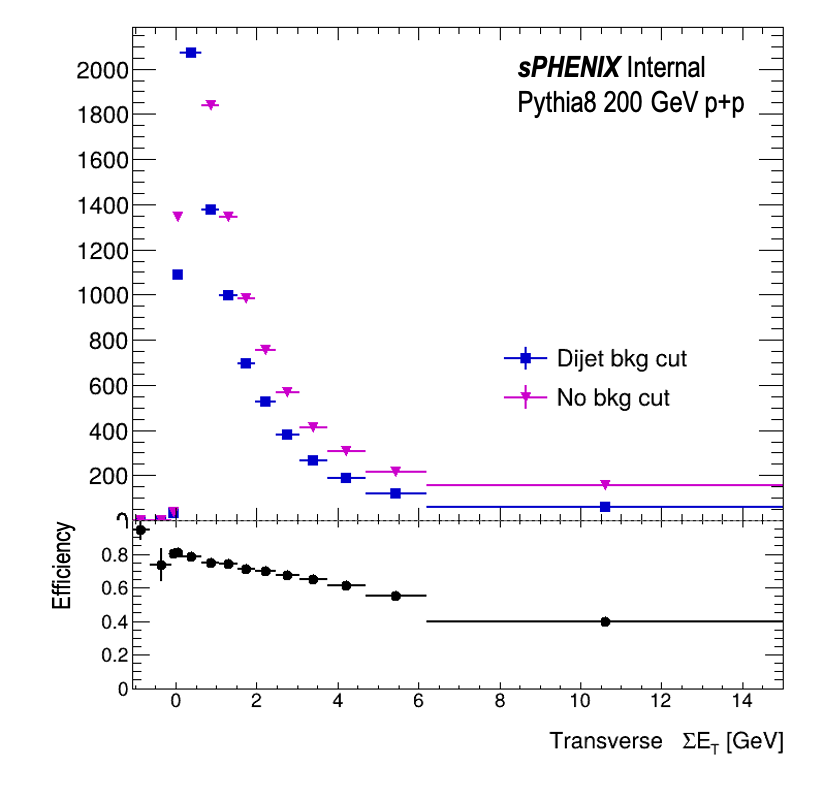
\includegraphics[width=0.48\linewidth]{figures/chapter5/dijet_bkg_cut_efficiency.png}
    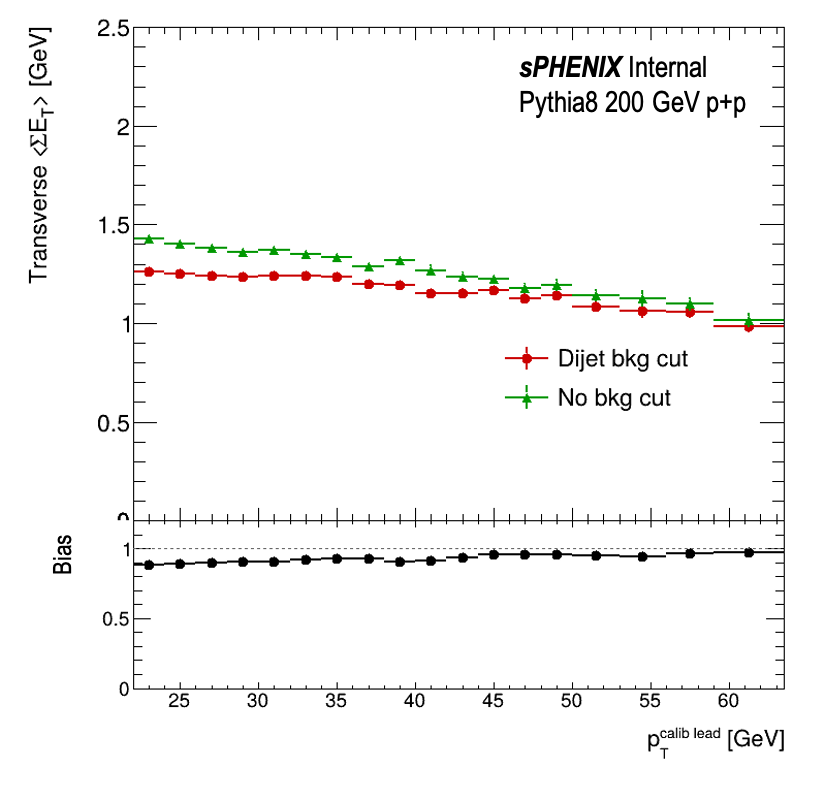
\includegraphics[width=0.48\linewidth]{figures/chapter5/dijet_bkg_cut_bias.png}
    \caption{Effect of the dijet cut on the transverse region $E_{T}$ distribution in the \pythia simulation dataset. 
    The left plot shows the efficiency of the dijet background cut application on the reco level transverse region $E_{T}$ distribution.
    The right plot shows the bias on the reco level $\langle \Sigma E_{T} \rangle$ as a function of calibrated reco leading jet $p_{T}$.}
    \label{fig:sim_dijet_bkg_tr_et}
\end{figure}
\begin{figure}
    \centering
    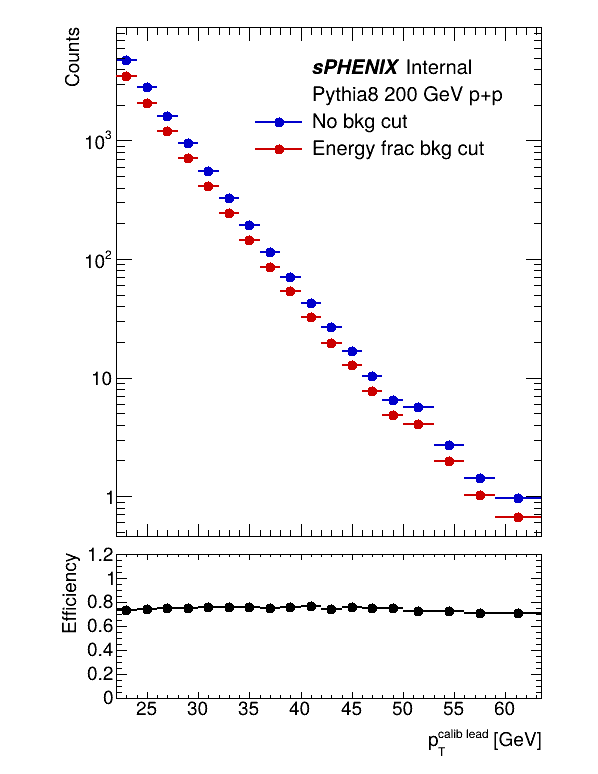
\includegraphics[width=0.5\linewidth]{figures/chapter5/efrac_bkg_cut_jetpt_efficiency.png}
    \caption{Effect of the energy fraction cut on the reconstructed leading jet $p_{T}$ distribution for inclusive jets in the analysis measurement range. (Top) Leading jet yield for inclusive jet events with and without the energy fraction cut. (Bottom) Efficiency of background cut application on jet yield in inclusive jet events for energy fraction cut used in inclusive jet analysis.} 
    \label{fig:sim_efrac_bkg_jetpt}
\end{figure}

\subsection{Data-Driven Jet Background Timing Cuts}
\label{sec:data_jet_timing}

Additional background rejection cuts are applied to both the inclusive jet and dijet samples to remove additional jet backgrounds not accounted for in the energy fraction cut or the requirement of a dijet event, respectively.
For the dijet analysis, two additional data-driven background cuts are applied. The first is on the leading jet time and second is on the time difference between the leading and subleading jet in the event~\cite{tf1_note}. 
The inclusive jet analysis also uses two additional data-driven background cuts. The ifrst is on the leading jet time, similar to the dijet analysis case, and the second is on the time difference between the leading jet and the MBD since a subleading jet may not be available in the inclusive jet case. Table~\ref{tab:jet_background_cuts} outlines the full set of jet background cuts applied to the inclusive jet and dijet analyses respectively.

\begin{table}[]
    \centering
    \begin{tabular}{c|c}
        \multicolumn{2}{c}{Inclusive Jet Events} \\
        \hline
        Cut Name & Application \\
        \hline
        E fraction cut & EMCal(10-90\%)/IHCal(0-90\%)/OHCal(10-90\%) E frac on lead jet \\
        Leading jet time cut & Require lead jet time in $[-8,4]$ ns \\
        Lead jet--MBD time diff cut & Require lead jet--MBD $\Delta t$ in $[-5,1]$ ns \\
    \end{tabular} \\
    \bigskip \bigskip
    \begin{tabular}{c|c}
        \multicolumn{2}{c}{Dijet Events} \\
        \hline
        Cut Name & Application \\
        \hline
        Dijet cut & Require $E_{\mathrm{sub}}/E_{\mathrm{lead}}>0.3$, $\Delta\phi>\Delta\phi_{\mathrm{min}} = 3\pi / 4$ \\
        Leading jet time cut & Require lead jet time in $[-8,4]$ ns \\
        Lead--sublead jet time diff cut & Require lead--sublead jet $\Delta t$ in $[-3,3]$ ns \\
    \end{tabular}
    \caption{Outline of jet background cuts applied to inclusive jet (top) and dijet (bottom) analyses respectively.}
    \label{tab:jet_background_cuts}
\end{table}

Detailed information on the development and investigation of this additional jet--MBD time difference cut is included in Appendix~\ref{sec:jet_mbd_time_bkg_cut}, while an example of the jet--MBD time difference distribution with cut bounds shown as well as the cut's efficiency and purity determination are included below.
The cut efficiency and purity are extracted by fitting the leading jet time and jet--MBD time distributions with a Gaussian plus constant background fit. 
The extracted signal and signal + background distributions are shown in Figure~\ref{fig:lead_jet_time_mbd_time_cut}.
As shown in Figure~\ref{fig:lead_jet_time_mbd_time_cut} (left), the leading jet timing window of $[-8,4]$~ns is used for the signal region. The jet--MBD time difference distribution is shown in Figure~\ref{fig:lead_jet_time_mbd_time_cut} (right), here a $\Delta t_{\mathrm{jet-MBD}}$ requirement of $[-5,1]$~ns is used for the signal region. 
The small tail in the $\Delta t_{\mathrm{jet-MBD}}$ distribution above 1~ns is attributed primarily to pileup.

\begin{figure}
    \centering
    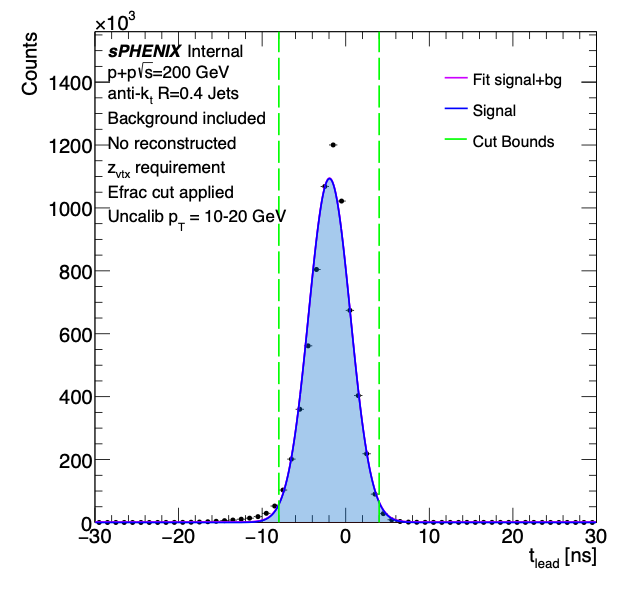
\includegraphics[width=0.48\linewidth]{ueinpp/Figures/jet_bkg_cuts/lead_jet_time_cut.png}
    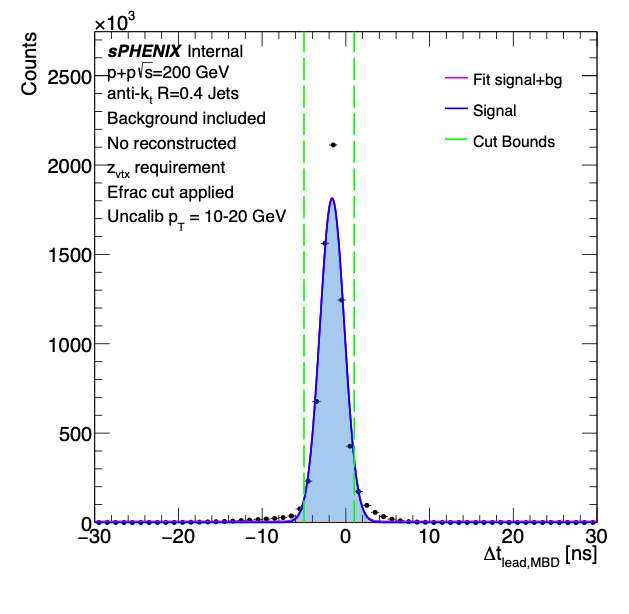
\includegraphics[width=0.48\linewidth]{ueinpp/Figures/jet_bkg_cuts/lead_jet_mbd_time_cut.png}
    \caption{Leading jet time (left) and leading jet--MBD time (right) distributions for events with leading jet $p_{T} = 10-20$ GeV and passing the "energy fraction" background cut. Extracted signal and signal + background distributions are shown within the cut window. The cut efficiency and purity are extracted from these signal and signal + background distributions.}
    \label{fig:lead_jet_time_mbd_time_cut}
\end{figure}

The timing cut efficiencies are determined as a function of leading jet $p_{T}$ and shown in Figure~\ref{fig:timing_cut_efficiencies}.
The jet timing cut efficiencies are around 98\% for the nominal leading jet time and jet--MBD time cuts and above 99\% for the variations of the nominal cuts which widen the timing windows by 1~ns.
The purity of the timing cuts is also determined as a function of leading jet $p_{T}$ and shown in Figure~\ref{fig:timing_cut_purity}.
The timing cuts have a very high purity ($>$99\%) for all but the last leading jet $p_{T}$ bin where the results are statistics limited.
The addition of these timing cuts, which have high efficiency and purity, allows for the removal of the small subset of background events that pass the stricter but less efficient energy fraction cut or dijet requirement used in the inclusive jet and dijet analyses, respectively.

\begin{figure}
    \centering
    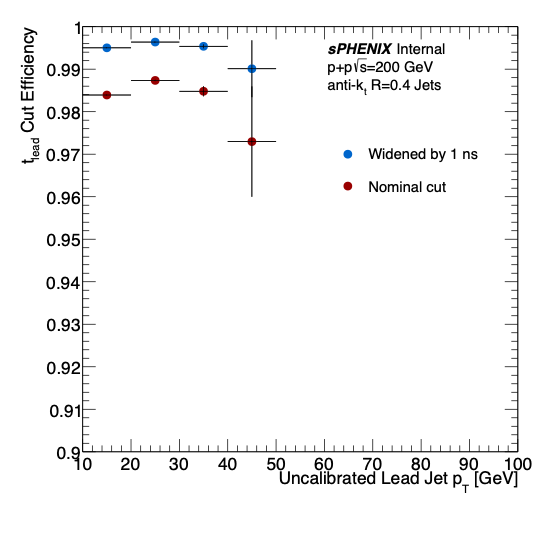
\includegraphics[width=0.48\linewidth]{ueinpp/Figures/jet_bkg_cuts/lead_time_cut_efficiency.png}
    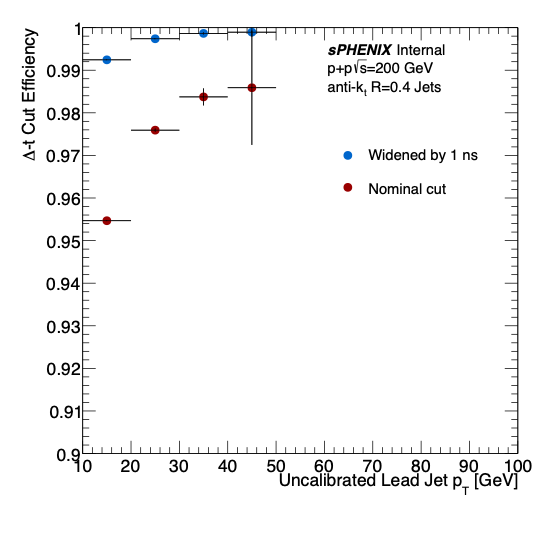
\includegraphics[width=0.48\linewidth]{ueinpp/Figures/jet_bkg_cuts/deltat_cut_efficiency.png}
    \caption{Timing cut efficiency as a function of leading jet $p_{T}$ for events passing the "energy fraction" background cut and the data-driven leading jet time + jet--MBD time cuts.}
    \label{fig:timing_cut_efficiencies}
\end{figure}

\begin{figure}
    \centering
    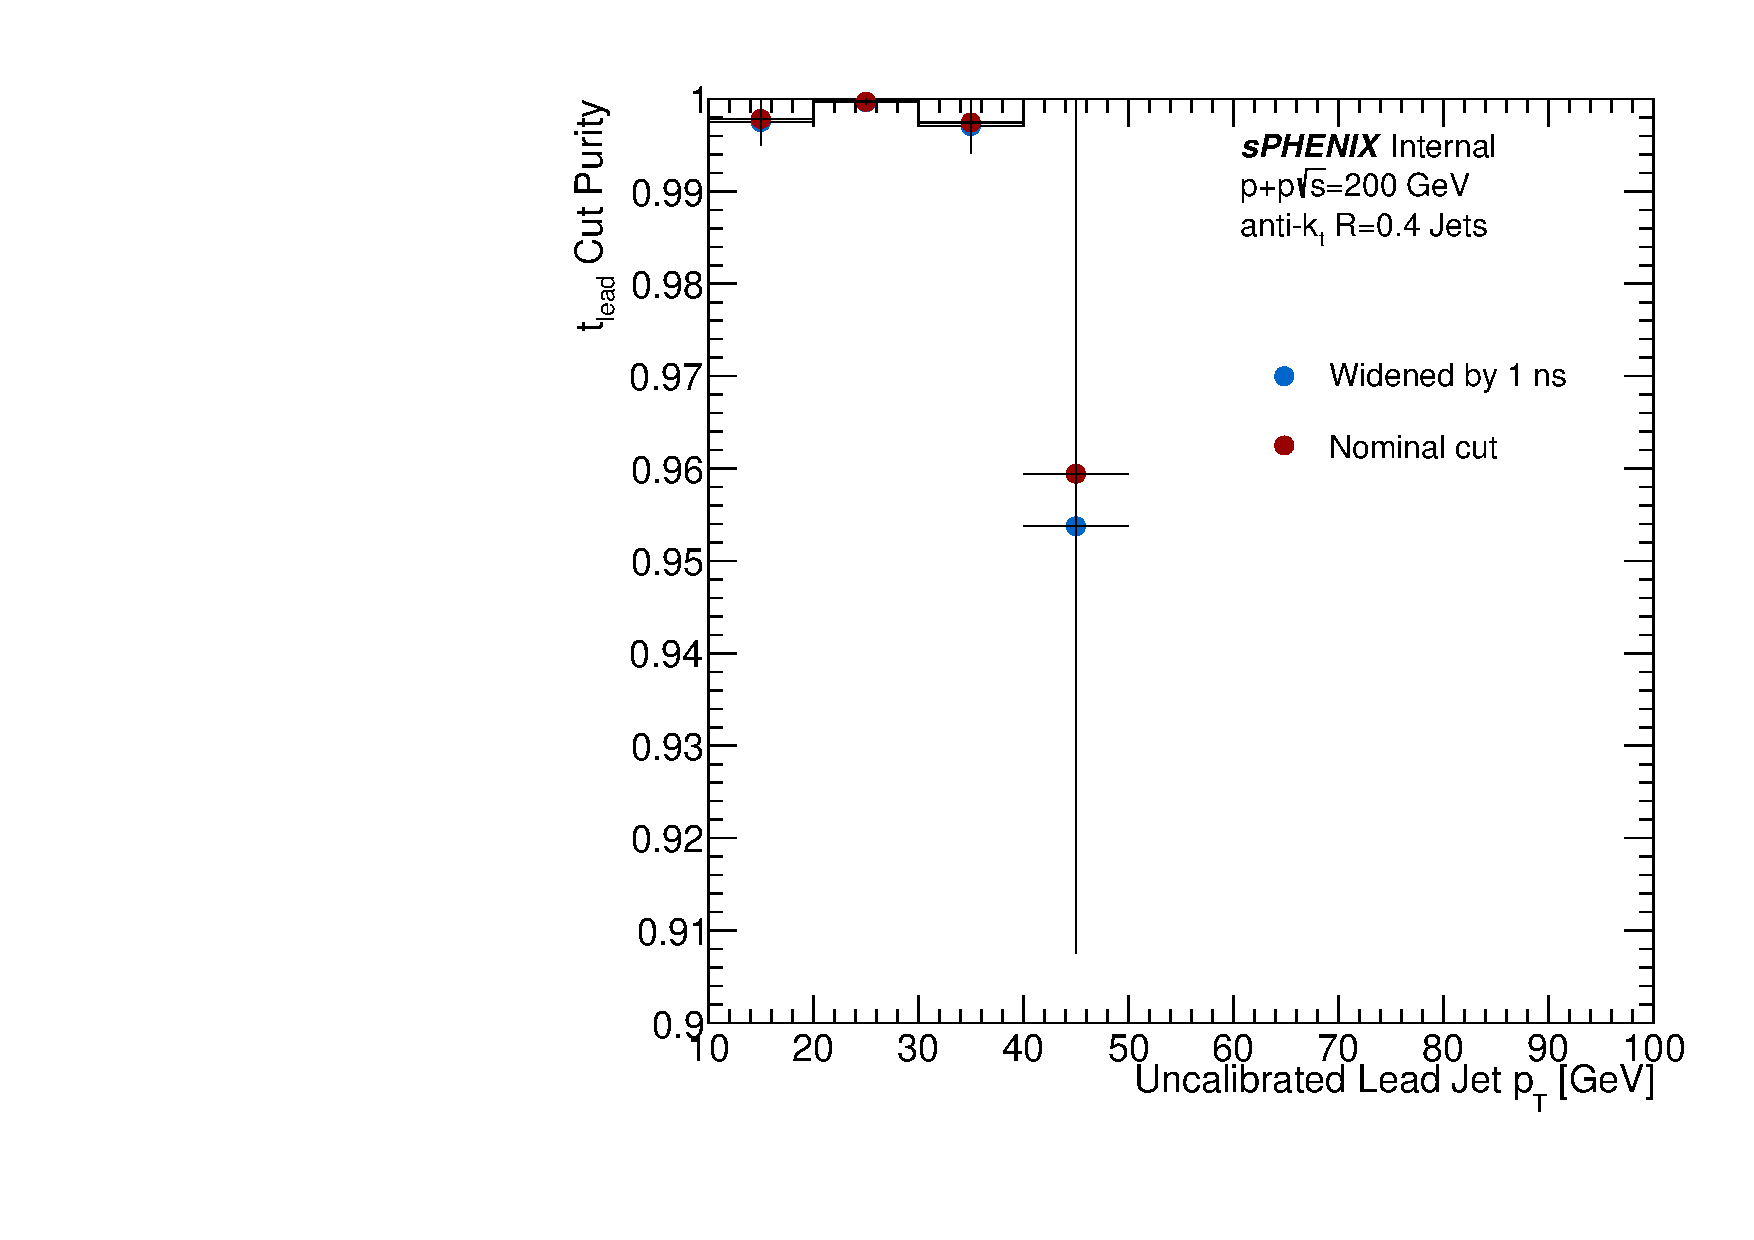
\includegraphics[width=0.48\linewidth]{ueinpp/Figures/jet_bkg_cuts/lead_time_cut_purity.pdf}
    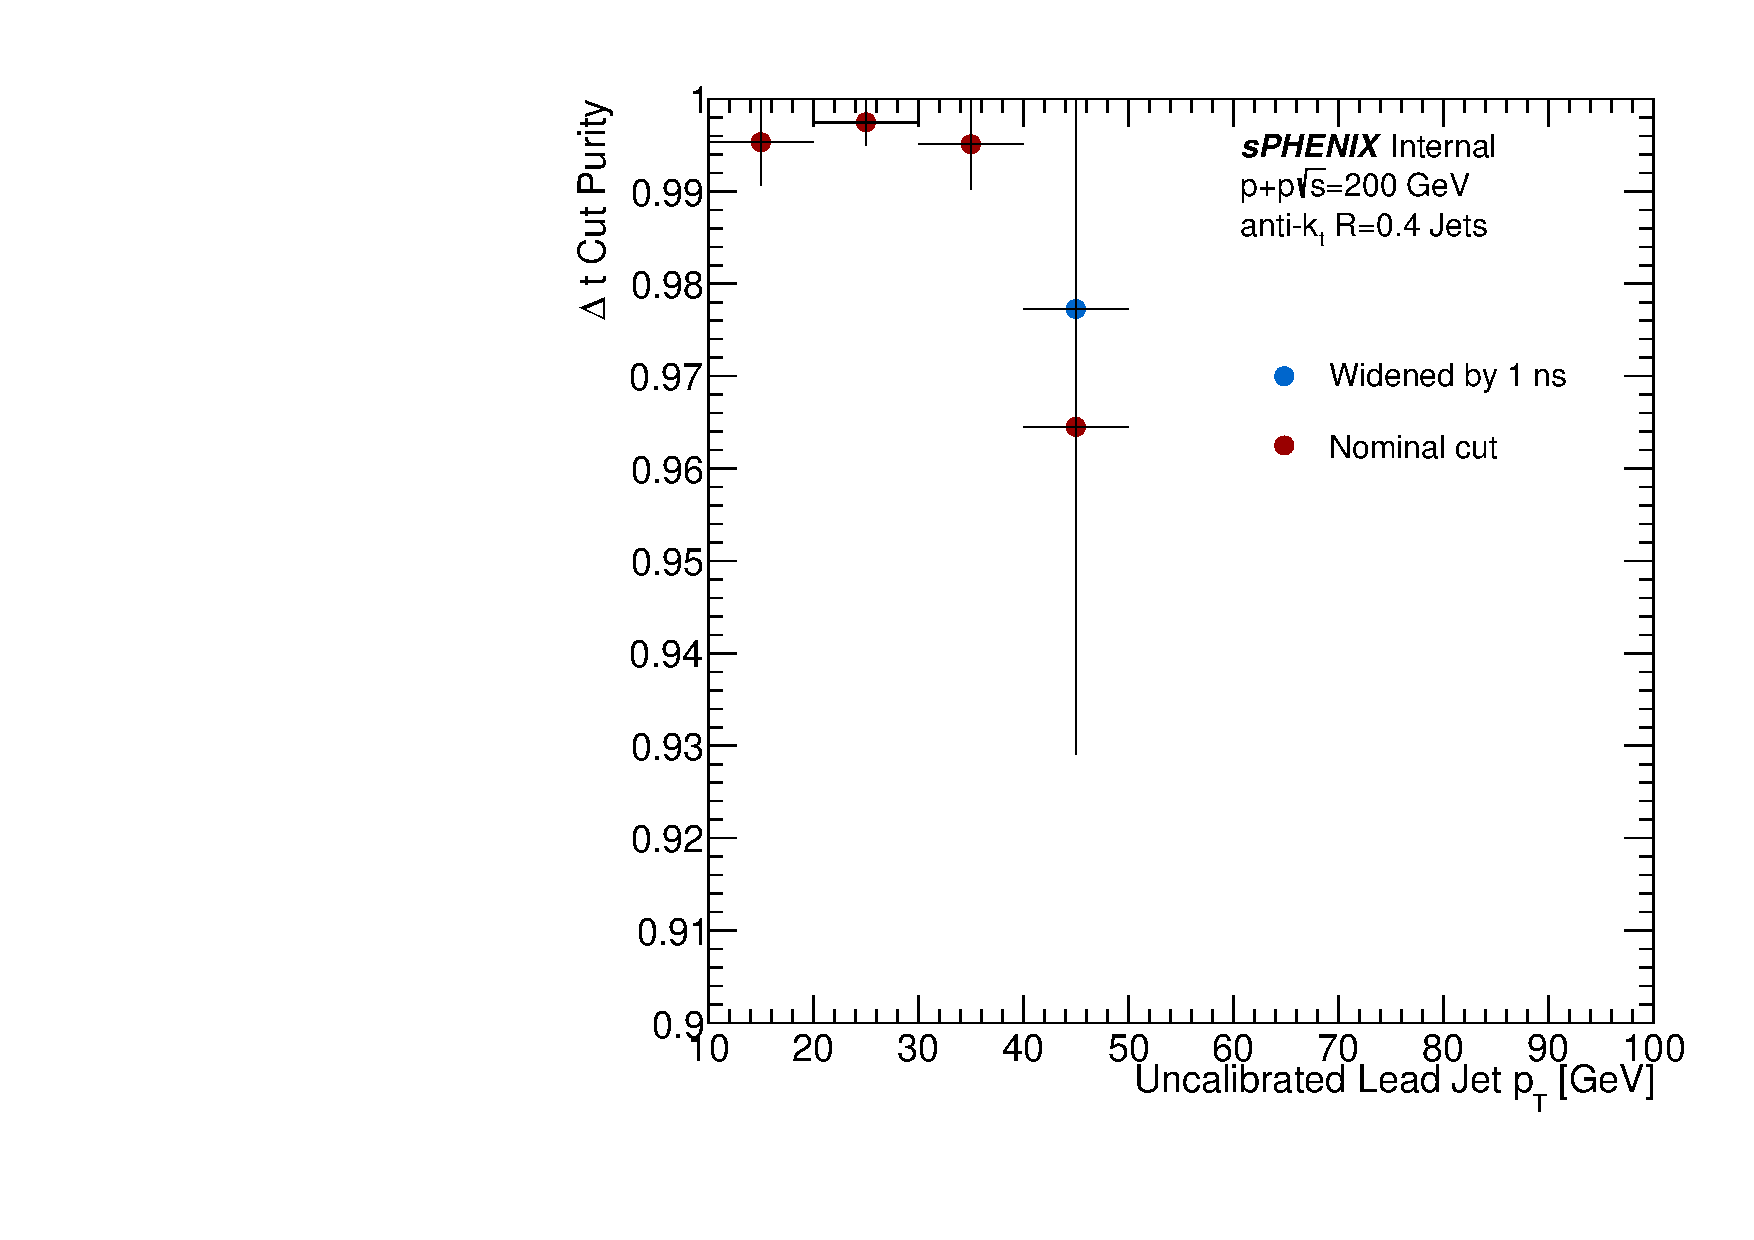
\includegraphics[width=0.48\linewidth]{ueinpp/Figures/jet_bkg_cuts/deltat_cut_purity.pdf}
    \caption{Timing cut purity as a function of leading jet $p_{T}$ for events passing the "energy fraction" background cut and the data-driven leading jet time + jet--MBD time cuts.}
    \label{fig:timing_cut_purity}
\end{figure}

